\documentclass{beamer}
\usepackage[latin1]{inputenc}
%\setbeamercovered{transparent}
\usetheme{Warsaw}
\title[Virtualization vulnerabilites]{Virtualization vulnerabilities\\
Past and future}
\author{Yann LEGER - Juan Sebastian PENA RODRIGUEZ}
\institute{Epitech -- UCSD}
\date{March 19, 2012}
\begin{document}
\AtBeginSection[]
{
  \begin{frame}<beamer>
    \frametitle{Layout}
    \tableofcontents[currentsection,currentsubsection]
  \end{frame}
}

\begin{frame}
\titlepage
\end{frame}

\section{Virtualization in the industry}
\begin{frame}{Why virtualization ?}
	\begin{itemize}
	\item Server consolidation
	\item[$\Rightarrow$] \emph{Better usage of ressources/Mutualization}\\
	\item[$\Rightarrow$] \emph{Reduce CAPEX (CAPital EXpense)}\\
	\item Flexibility
	\item[$\Rightarrow$] \emph{Live migration}\\
	\item[$\Rightarrow$] \emph{Reduce physical modification need}\\
	\item Isolation
	\item[$\Rightarrow$] \emph{Performance isolation}\\
	\item[$\Rightarrow$] \emph{\alert{Security isolation}}\\
	\end{itemize}
\end{frame}

\begin{frame}{Virtualization adoption}
	\begin{block}{Statistics}
		23\% of installed applications were running in a VM in 2010.\\
		$\Rightarrow$ \emph{Estimation says that 48\% of installed applications will run on a VM by 2012.}\\
	\end{block}
	\begin{block}{Business creation}
		Cloud computing is powered by virtualization\\
		$\Rightarrow$\emph{Amazon EC2, Rackspace, IaaS, PaaS, SaaS...}\\
	\end{block}
\end{frame}

\section{Security}
\begin{frame}{The threat is real}
	\begin{center}
	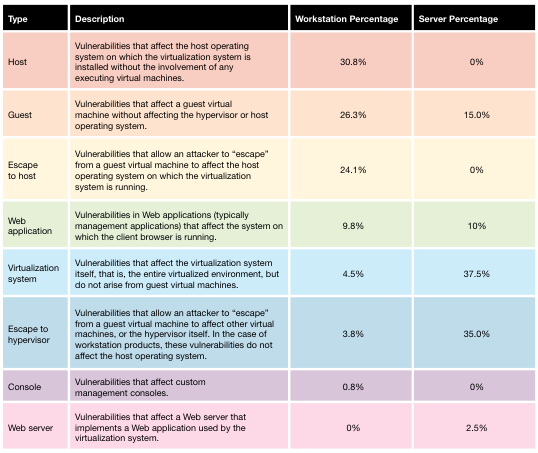
\includegraphics[scale=0.3]{table-vuln}
	\end{center}
	Source : \emph{IBM X-Force 2010 Mid-Year Trend and Risk Report}
\end{frame}

\begin{frame}{CVE Statistics}
	\begin{itemize}
	\item 500 CVE entries related to VMWare
	\item[$\Rightarrow$]\emph{Many products and many third party libraries}\\
	\item 41 CVE entries related to QEMU KVM
	\item[$\Rightarrow$]\emph{Doesn't include Linux/third party libraries bugs}\\
	\item 68 CVE entries related to Xen
	\item[$\Rightarrow$]\emph{Doesn't include Linux/third party libraries bugs}\\
	\end{itemize}
\end{frame}

\begin{frame}{VMware Workstation versus QEMU-KVM}
	\begin{block}{VMware Workstation}
	\begin{itemize}
	\item Many vulnerabilities due to extended functionalities
	\item Difficult to gather information due to the absence of open bug tracker
	\end{itemize}
	\end{block}
	\begin{block}{QEMU-KVM}
	\begin{itemize}
	\item Codebase is really small
	\item Difficult to gather information due to the bad tagging in the bug tracker
	\item \emph{Nelson Elhage} breaked out of KVM (demonstrated at DEFCON and Back Hat)
	\end{itemize}
	\end{block}
\end{frame}

\section{Trends}
\begin{frame}{Software improvements}
	\begin{itemize}
	\item Reducing Trusted Computing Base (TCB)
	\item[$\Rightarrow$] \emph{Previous work on Xen attempted to reduce the TCB}\\
	\item Using operating system mechanism when possible
	\item[$\Rightarrow$]\emph{AppArmor on Ubuntu, SELinux on RedHat/CentOs, GRSec with kernel-level virtualization}\\
	\end{itemize}
\end{frame}

\begin{frame}{Hardware improvements}
	\begin{itemize}
	\item Intel VT-x and AMD-V instruction sets
	\item[$\Rightarrow$] \emph{Avoid binary translation and Guest OS modification}\\
	\item Intel EPT and AMD RVI instruction set
	\item[$\Rightarrow$] \emph{Virtualization of MMU, no need to trap into hypervisor on page update}\\
	\item Intel VT-d and AMD-V for IOMMU virtualization
	\item[$\Rightarrow$] \emph{Avoid emulated/paravirtualized devices, allow to dedicate a device to a virtual machine}\\
	\item SR-IOV allow device virtualization
	\item[$\Rightarrow$] \emph{Up to 128 virtual network card with one physical device (e.g. Cisco Palo)}
	\end{itemize}
	\alert{Reduce code quantity and thus bugs}
\end{frame}

\begin{frame}{Conclusion}
	\begin{itemize}
	\item Many security improvements from reduction of the code base
	\item Hardware assisted virtualization help reduce the trusted computing base
	\item Virtualization is improving fast and has become a powerful tool
	\end{itemize}
\end{frame}

\begin{frame}{Questions ?}
		\begin{center}
		Questions ?
		\end{center}
\end{frame}

\end{document}
